\renewcommand*{\arraystretch}{1.1}

\noindent\begin{tabularx}{17cm}{|p{1.95cm}|X|}
	\hline
	workload    & Interactive / update \\ \hline
%
	query       & 1 \\ \hline
%
	title       & Add Person \\ \hline
%
    pattern     & \hfill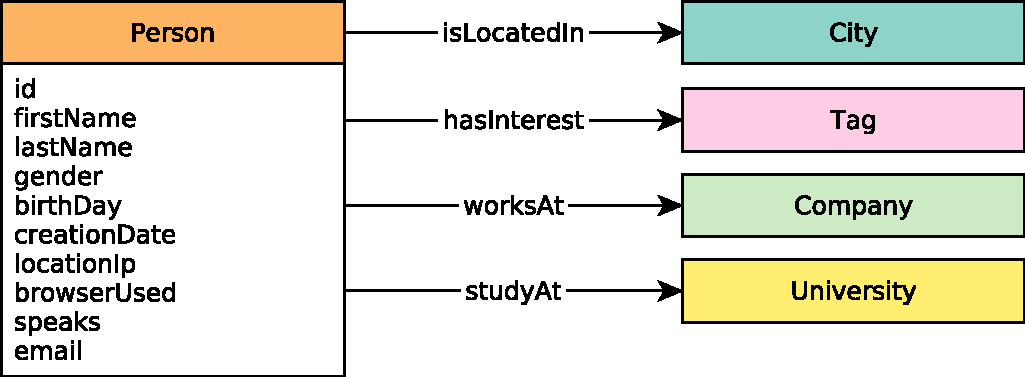
\includegraphics[scale=\patternscale,margin=0cm .2cm]{patterns/interactive-update-01}\hfill\vadjust{} \\ \hline
%
	description & Add a Person to the social network.
 \\ \hline
%
	
%
	parameters  &
	\vspace{1.1ex}{\begin{tabularx}{14.2cm}{|c|M|m{2cm}|Y|} \hline
	\cellcolor{black!70} \color{white} $\mathsf{1}$ & \varname{Person.id} & \cellcolor{gray!20} \vartype{ID} &  \\ \hline
	\cellcolor{black!70} \color{white} $\mathsf{2}$ & \varname{Person.firstName} & \cellcolor{gray!20} \vartype{String} &  \\ \hline
	\cellcolor{black!70} \color{white} $\mathsf{3}$ & \varname{Person.lastName} & \cellcolor{gray!20} \vartype{String} &  \\ \hline
	\cellcolor{black!70} \color{white} $\mathsf{4}$ & \varname{Person.gender} & \cellcolor{gray!20} \vartype{String} &  \\ \hline
	\cellcolor{black!70} \color{white} $\mathsf{5}$ & \varname{Person.birthDay} & \cellcolor{gray!20} \vartype{Date} &  \\ \hline
	\cellcolor{black!70} \color{white} $\mathsf{6}$ & \varname{Person.creationDate} & \cellcolor{gray!20} \vartype{DateTime} &  \\ \hline
	\cellcolor{black!70} \color{white} $\mathsf{7}$ & \varname{Person.locationIp} & \cellcolor{gray!20} \vartype{String} &  \\ \hline
	\cellcolor{black!70} \color{white} $\mathsf{8}$ & \varname{Person.browserUsed} & \cellcolor{gray!20} \vartype{String} &  \\ \hline
	\cellcolor{black!70} \color{white} $\mathsf{9}$ & \varname{Person-isLocatedIn->City.id} & \cellcolor{gray!20} \vartype{ID} &  \\ \hline
	\cellcolor{black!70} \color{white} $\mathsf{10}$ & \varname{Person.speaks} & \cellcolor{gray!20} \vartype{\{ String \}} &  \\ \hline
	\cellcolor{black!70} \color{white} $\mathsf{11}$ & \varname{Person.emails} & \cellcolor{gray!20} \vartype{\{ String \}} &  \\ \hline
	\cellcolor{black!70} \color{white} $\mathsf{12}$ & \varname{Person-hasInterest->Tag.id} & \cellcolor{gray!20} \vartype{\{ ID \}} &  \\ \hline
	\cellcolor{black!70} \color{white} $\mathsf{13}$ & \varname{\{ Person-studyAt->University.id, Person-studyAt->.classYear \}} & \cellcolor{gray!20} \vartype{\{ID, 32-bit Integer\}} &  \\ \hline
	\cellcolor{black!70} \color{white} $\mathsf{14}$ & \varname{\{ Person-workAt->Company.id, Person-workAt->.workFrom \}} & \cellcolor{gray!20} \vartype{\{ID, 32-bit Integer\}} &  \\ \hline
	\end{tabularx}}\vspace{1.1ex} \\ \hline
%
	
%
	%
	%
	%
\end{tabularx}